\documentclass[11pt]{article}

\usepackage[utf8]{inputenc}
\usepackage[T1]{fontenc}
\usepackage[margin=1in]{geometry}
\usepackage{amsmath}
\usepackage{graphicx}
\usepackage{booktabs}
\usepackage{authblk}
\usepackage{hyperref}
\graphicspath{{../figures/}{figures/}{./}}

\title{Cadence, CubeSats, and Certainty: How Constellation Size Affects Reverberation-Mapped Black Hole Mass Uncertainty}
\author{Aisha Shermatova}
\date{}

\begin{document}

\maketitle

% NOTE: every number, table and figure in this version is generated by the accompanying code
% (paper/make_paper.py reads results/*.json). Re-run the simulations and this script to regenerate.

\begin{abstract}
Active galactic nuclei (AGN), the actively accreting subset of supermassive black holes, offer one of the few ways to measure a black hole's mass without resolving it directly, through reverberation mapping, which measures the delay between variability in the central continuum and the broad-line region (BLR) gas that echoes it. Reverberation mapping requires sustained, high-cadence monitoring that is expensive and hard to schedule on shared telescopes, limiting how many AGN can be studied. We ask how the number of satellites in a low-cost CubeSat constellation affects the uncertainty of reverberation-mapped lags and black hole masses for bright AGN with BLR lags of days to weeks. Using synthetic Damped Random Walk light curves and Interpolated Cross-Correlation Function (ICCF) lag recovery, we first run a controlled experiment in which cadence scales with constellation size at fixed photometric noise. Fractional lag uncertainty falls from 41.4\% to 18.5\% between 3 and 12 satellites (Welch's $t$-tests, $p<0.001$), roughly as $N^{-0.65}$ with no plateau, and a binning test shows that the gain comes from averaging photometric noise over more epochs rather than from finer sampling. We then replace the assumed noise and cadence by a mission-level model: a photon budget for a 10-cm CubeSat photometer, a precessing orbit (J2 nodal regression of 4.77 degrees per day), a real solar ephemeris, ground-station bandwidth, and six catalogued reverberation-mapping AGN. A single satellite already collects about 127 exposures per day, so the constellation size matters mainly when the data are photon-starved or weakly variable: for a V = 17 target of 4\% variability the fractional lag uncertainty falls from 37.7\% with one satellite to 8.0\% with twelve, whereas for a V = 15 target of 10\% variability it is near 3.4\% regardless of constellation size. Solar exclusion depends strongly on ecliptic latitude, from no exclusion for the southernmost target to gaps of up to 88 days at low ecliptic latitude, and a seasonal gap biases the recovered lag and removes most of the benefit of additional satellites. Target selection and campaign timing therefore matter at least as much as constellation size.

\vspace{0.5em}
\noindent\textbf{Keywords:} Reverberation mapping, Damped Random Walk, Interpolated Cross-Correlation Function, CubeSat constellation, black hole mass uncertainty
\end{abstract}

\section{Introduction}

Direct imaging campaigns have confirmed the presence of supermassive black holes at the centers of galaxies, most notably the Event Horizon Telescope's images of the black hole shadows at the centers of M87 (Event Horizon Telescope Collaboration et al., 2019) and the Milky Way (Event Horizon Telescope Collaboration et al., 2022), and how the black hole grows helps shape how the galaxy evolves (Lewin, 2025). Studying the region close enough to a black hole to observe its accretion disk directly reveals both the black hole's mass and the physical conditions of the surrounding accreting gas, but this region is too small for even the best telescopes to resolve directly. Reverberation mapping gets around this by trading spatial resolution for time resolution: it measures the delay between light from near the black hole, which reaches the observer first, and light reprocessed by gas farther out in the broad line region (BLR), which arrives afterward (Gorjian et al., 2025). Tracking this delay lets astronomers infer the physical size of the BLR and, combined with the velocity of the gas, estimate the black hole's mass, one of the only ways to do so without ever resolving the black hole directly (Malik, 2023).

However, reverberation mapping is telescope-intensive and requires sustained monitoring over weeks or months. Furthermore, ultraviolet-capable facilities are scarce enough that only a small number of AGN have ever received the high-cadence coverage required by this technique (Gorjian et al., 2025). A four-year campaign monitoring 18 AGN found that a cadence of roughly one to three days, sustained for at least ninety days, produces reliable lag recovery for AGN with SMBH masses between $10^{7-8}\,M_\odot$ (Miller et al., 2026). Separate work shows that gaps in an observing window can meaningfully degrade lag recovery even when the total monitoring time is otherwise sufficient (Malik et al., 2022).

Small, low-cost satellites offer one possible way around the scheduling bottleneck that limits ground-based campaigns: a dedicated satellite does not compete with other observers for shared telescope time, so it can, in principle, monitor a single AGN continuously for as long as the science requires. Proposed missions such as the BHAGERA SmallSat are already being designed around this idea (Gorjian et al., 2025), and CubeSats more broadly are increasingly treated as legitimate tools for time-domain astrophysics rather than simply a cheaper substitute for real telescopes (Knapp \& Seager, 2018).

Small satellites are already used for astrophysics in the ultraviolet and optical, and flight heritage exists for the instrument class considered here: 6U CubeSats such as CUTE (a near-ultraviolet spectrograph) and SPARCS (an ultraviolet stellar-activity monitor), and larger small-mission concepts such as the wide-field ultraviolet time-domain telescope ULTRASAT. These missions motivate the 10--15 cm apertures and 6U--12U platforms adopted below.
% TODO(author): add proper references for CUTE, SPARCS and ULTRASAT (and any dedicated AGN reverberation-mapping CubeSat concept); verify the instrument descriptions against the mission papers.

This study investigates how the observation cadence achievable by a low-cost CubeSat constellation affects the uncertainty of reverberation-mapped black hole mass estimates for bright AGN with BLR lags of days to weeks.

Such a satellite constellation is only useful if the cadence it can realistically achieve can recover a reliable lag, and by extension, a reliable black hole mass. The reverberation mapping literature already treats cadence as a primary driver of measurement uncertainty rather than a minor detail (Malik et al., 2022; Miller et al., 2026), and the field's own rule of thumb calls for a cadence roughly five times finer than the lag being measured (Shablovinskaya et al., 2023). If a modest, low-cost constellation can approach the cadence, and therefore the precision, that currently requires scarce, expensive telescope time, the number of AGN studied using reverberation mapping can be greatly increased, addressing the same scalability problem that motivates multi-object reverberation mapping approaches on the ground (Malik, 2023).

We hypothesize that increasing the constellation size from 3 to 12 satellites improves observation cadence and reduces lag recovery uncertainty, but with diminishing returns as satellite count increases, since cadence improvements beyond roughly five times finer than the true lag are expected to yield progressively smaller gains in precision. Because cadence and photometric noise both depend on the instrument and the orbit, we also test the hypothesis in a mission-level model in which they are derived and not assumed.

The remainder of this paper is organized as follows: Section 2 describes the simulation methodology, Section 3 presents the controlled experiment, the estimator diagnostics, the astrophysical parameter sweeps, the photon budget, and the dynamic-orbit mission model, Section 4 discusses their implications and limitations, and Section 5 concludes.

\section{Methods}

\subsection{Research Design}

We built a simulation pipeline in Python that generates synthetic AGN light curves, samples them at the epochs a constellation of $N$ satellites could obtain, recovers a time lag from each sampled light curve, and converts the lag into a black hole mass uncertainty. Two experiments share this pipeline. The \emph{controlled experiment} fixes the photometric noise and sets the cadence to a nominal 2 days divided by $N$, so that constellation size is the only quantity that varies; because the number of epochs grows in proportion to $N$, it varies the sampling interval and the number of measurements together, and a binning test (Section~\ref{sec:diag}) separates the two. The \emph{mission experiment} replaces the assumed noise and cadence by quantities derived from a photon budget, a precessing orbit and catalogued targets (Sections~\ref{sec:instrument} and~\ref{sec:orbit}).

\subsection{Light Curve Simulation}

We generated synthetic AGN continuum light curves with the Damped Random Walk (DRW) model, the standard statistical description of quasar optical variability (Kelly et al., 2009). The continuum flux reverts toward its mean on a damping timescale $\tau_d$, with an asymptotic fractional rms amplitude $\sigma_V$. The fiducial values are $\tau_d = 50$ days and $\sigma_V = 4\%$, over a baseline of 120 days, evolved with the exact DRW update on a 0.05-day grid; the fiducial amplitude makes the intrinsic variability comparable to the 3\% photometric noise of the controlled experiment, a regime in which lag recovery is demanding. Section~\ref{sec:sweeps} sweeps $\tau_d$ from 20 to 200 days and $\sigma_V$ from 1\% to 15\%.
% TODO(author): an earlier draft stated a 20% amplitude. With this pipeline a 20% amplitude gives much smaller
% uncertainties (about 5% fractional lag error in a short test). Confirm the fiducial amplitude and regenerate if you change it (--amp).

The BLR response is the continuum convolved with a transfer function of mean lag 10 days (5 and 20 days in the sensitivity runs). The fiducial transfer function is a top-hat of width 4 days; we also test skewed log-normal transfer functions with standard deviations of 4 and 8 days (same mean lag), which broaden and skew the response as expected for extended BLRs. The line flux is scaled to half the continuum flux, a cosmetic choice that does not affect the correlation.

\subsection{Instrument and Photon Budget}
\label{sec:instrument}

In the mission experiment the photometric noise follows from a photon budget instead of a fixed percentage. For a target of magnitude $V$ observed through a band of width $\Delta\lambda$, the per-exposure fractional noise is
\begin{equation}
\frac{\sigma_F}{F} = \frac{\sqrt{S + B_{\mathrm{sky}} + B_{\mathrm{dark}} + n_{\mathrm{pix}} R^2}}{S},
\end{equation}
where $S$ is the number of target electrons, $B_{\mathrm{sky}}$ and $B_{\mathrm{dark}}$ are the sky and dark electrons inside the photometric aperture, $n_{\mathrm{pix}}$ is the number of aperture pixels and $R$ is the read noise. We use $1005$ photons s$^{-1}$ cm$^{-2}$ \AA$^{-1}$ at $V=0$, and a representative photometer: a 10~cm (6U) or 15~cm (12U) aperture with a 10\% obstruction, a total throughput of 0.55, a detector quantum efficiency of 0.8, 3$''$ pixels with a 2.5-pixel aperture radius, 3~e$^-$ read noise, a dark current of 0.1~e$^-$ s$^{-1}$ pixel$^{-1}$, and a combined zodiacal and stray-light background of 22 mag arcsec$^{-2}$. A dichroic splits the light into a 1000~\AA\ continuum channel and a 150~\AA\ line channel that are exposed simultaneously, so the line channel has fewer photons and therefore higher noise. Exposures last 120~s with a 60~s overhead (readout, settling and pointing) per epoch, giving a cycle time of 180~s. All of these are assumptions for a representative instrument and not the parameters of a specific flight design; line-channel contamination by continuum light is ignored.

An exposure is useful only if it reaches the ground. We assume 64~kB of on-board-extracted photometric windows per exposure and a 2~Mbps downlink to a single station ($40^{\circ}$N, $0^{\circ}$E, minimum elevation $10^{\circ}$), and we cap the number of exposures per time bin by the data volume that fits in the ground-station passes within that bin. Full-frame readout (16~MB per exposure) is tested as an alternative.

\subsection{Dynamic Orbital Model and Catalogued Targets}
\label{sec:orbit}

Constellations of $N$ satellites are evenly phased in one circular orbit at 500~km altitude and $51.6^{\circ}$ inclination, with the right ascension of the ascending node initially at $0^{\circ}$. All geometry is evaluated every 60~s in an Earth-centred inertial equatorial frame. The orbital plane precesses at the $J_2$ nodal regression rate, $\dot\Omega = -\tfrac{3}{2} J_2 (R_\oplus/a)^2 n \cos i$, which is 4.77 degrees per day for this orbit, so the plane rotates by $360^{\circ}$ in about 75 days and the viewing geometry and eclipse fraction change over a 120-day campaign. The Sun's position comes from a low-precision solar ephemeris (Vallado, 2013) starting on 1 January 2026. Three constraints are applied per satellite: (i) \emph{Earth occultation}, blocking the sightline when its closest approach to Earth's centre lies inside Earth's radius in the direction of observation; (ii) \emph{Sun avoidance}, blocking observation when the target is within $45^{\circ}$ of the Sun (a representative baffle limit; real designs vary roughly $40$--$90^{\circ}$); and (iii) \emph{eclipse}, using a cylindrical Earth shadow, with a 10-minute thermal recovery after each eclipse exit. Ground-station bandwidth is handled as described above. A constellation can observe whenever at least one satellite satisfies all constraints.

Targets are six well-studied reverberation-mapping AGN spanning ecliptic latitudes from $+37^{\circ}$ to $-59^{\circ}$: NGC~5548, NGC~4151, NGC~7469, Mrk~509, NGC~3783 and Fairall~9, with J2000 positions from the standard catalogues.
% TODO(author): verify the RA/Dec values in cubesat_rm/orbit_dynamic.py against SIMBAD or NED before publication.
To isolate geometry, all targets are given the same fiducial magnitude $V = 15$ (actual magnitudes differ); magnitude is varied separately. To quantify how campaign timing affects the solar exclusion, we also compute the number of excluded days for 120-day campaigns starting every 30 days through the year.

\subsection{Observational Sampling}

In the controlled experiment the epochs are uniformly spaced at $2\,\mathrm{d}/N$ with a small random jitter ($\pm10\%$ of the cadence) and Gaussian photometric noise of 3\% (6\% and 10\% in the sensitivity runs). In the mission experiment the exposures are grouped into 0.5-day bins; each bin with at least one exposure becomes an epoch at the bin centre, with fractional noise equal to the per-exposure noise divided by the square root of the number of exposures in the bin, separately for the continuum and line channels. Light curves with fewer than 20 epochs are treated as too sparse.

\subsection{Lag Recovery and Uncertainty}

Lags are recovered with the Interpolated Cross-Correlation Function (ICCF) method (White \& Peterson, 1994; Peterson et al., 2004) on a grid of trial lags from $-5$ to 40 days in 0.5-day steps. For each trial lag, each light curve is interpolated onto the other's epochs, shifted by the lag, and the correlation coefficients of both directions are averaged. The peak lag is the lag of maximum correlation, and the centroid lag is the correlation-weighted mean of all trial lags with correlation above 80\% of the peak. Standard practice often restricts the centroid to the contiguous region around the peak; Section~\ref{sec:diag} shows that this choice changes the recovered uncertainties substantially when the correlation is modest.

Uncertainties use flux randomization/random subset sampling (FR/RSS; Peterson et al., 1998, 2004): in each of 1200 Monte Carlo trials we resample each light curve with replacement, discard duplicates, perturb each retained flux by a draw from its error bar and recompute the centroid; the standard deviation of the resulting distribution is the lag uncertainty of that realization.\footnote{We tested whether the number of Monte Carlo trials affected the stability of this estimate by repeating the FR/RSS procedure 15 times at each of four trial counts (150, 300, 600, 1200) for each constellation size. The mean estimate was stable, but its spread narrowed through 1200 trials, motivating the choice of 1200 trials. The test is available as \texttt{mc-convergence} in the code repository.}
% TODO(author): run `python -m cubesat_rm mc-convergence` and confirm this footnote still describes the result.
To account for the randomness of the DRW process, the full procedure is repeated over independent realizations (100 for the baseline, 30 for the sensitivity, sweep and mission runs, and 100 with 600 trials for the diagnostics). The recovered lag of a realization is the mean of its FR/RSS distribution, and the fractional lag uncertainty is the mean lag uncertainty divided by the mean recovered lag.

\subsection{Mass Conversion}

Each recovered lag is converted to a black hole mass with the virial relation
\begin{equation}
M_{\mathrm{BH}} = f \, \frac{c \, \tau \, \Delta V^2}{G},
\label{eq:virial}
\end{equation}
where $\tau$ is the recovered lag, $\Delta V$ the BLR velocity width and $f$ the virial factor. We adopt $f = 1.4$ (Onken et al., 2004) and $\Delta V = 3000$~km/s with a 10\% uncertainty. Because this study compares relative uncertainties, the fixed multiplier $f$ does not affect the comparison. Since $M_{\mathrm{BH}} \propto \tau\,\Delta V^2$, the fractional mass uncertainty is
\begin{equation}
\frac{\sigma_M}{M} = \sqrt{\left(\frac{\sigma_\tau}{\tau}\right)^2 + \left(2\,\frac{\sigma_{\Delta V}}{\Delta V}\right)^2},
\end{equation}
so the assumed velocity uncertainty sets a floor of 20\%.

\subsection{Sensitivity Analysis, Parameter Sweeps and Estimator Diagnostics}

The sensitivity analysis repeats the controlled experiment with true lags of 5, 10 and 20 days and noise levels of 3\%, 6\% and 10\% (30 realizations, 1200 trials; the 10-day, 3\% case is common to both). The parameter sweeps vary one astrophysical parameter at a time: $\tau_d$, $\sigma_V$ and the transfer function, each with uniform sampling and with a 36-day seasonal gap (days 41--77, the Sun-exclusion window of the earlier fixed-geometry model) removed from the epochs (30 realizations, 400 trials). The diagnostics compare the ICCF centroid of the unperturbed light curves with the known true lag, reporting the bias with a 95\% bootstrap interval, the root-mean-square error, the $1\sigma$ coverage of the FR/RSS interval and the gross-failure rate (more than 5 days from the truth); they repeat the analysis with the contiguous-region centroid, and a binning test averages the 12-satellite data in groups of four epochs, which gives the 3-satellite cadence at half the photometric noise.

\section{Results}

\subsection{Controlled Experiment: Lag and Mass Uncertainty Versus Constellation Size}

Table~\ref{tab:baseline} summarizes the controlled experiment (true lag 10~days, 3\% noise, 100 realizations). Fractional lag uncertainty decreases monotonically from 41.4\% to 18.5\% as the constellation grows from 3 to 12 satellites, and fractional mass uncertainty from 46.0\% to 27.2\%.

\begin{table}[htbp]
\centering
\small
\caption{Recovered lag and mass uncertainty by constellation size (true lag = 10.0 days; 100 realizations, 1200 MC trials per realization). SEM is the standard error of the mean lag uncertainty. Fractional lag error is the mean lag $\sigma$ divided by the mean recovered lag.}
\label{tab:baseline}
\resizebox{\textwidth}{!}{%
\begin{tabular}{@{}ccccccc@{}}
\toprule
Satellites & Cadence (days) & Recovered lag (days) & Lag $\sigma$ (days) & SEM (days) & Fractional lag error & Fractional mass error \\
\midrule
3 & 0.667 & 10.77 & 4.46 & 0.197 & 41.4\% & 46.0\% \\
6 & 0.333 & 10.60 & 2.80 & 0.164 & 26.4\% & 33.1\% \\
12 & 0.167 & 9.75 & 1.80 & 0.129 & 18.5\% & 27.2\% \\
\bottomrule
\end{tabular}}
\end{table}

The mean recovered lags differ from the true lag by +0.77, +0.60 and -0.25 days; normalizing the lag uncertainties by the true lag instead gives 44.6\%, 28.0\% and 18.0\%. Pairwise Welch's $t$-tests of the lag uncertainty are all significant (3 vs. 6: $t=6.50$, $p<0.0001$; 6 vs. 12: $t=4.78$, $p<0.0001$; 3 vs. 12: $t=11.30$, $p<0.0001$), but because $p$-values from simulations shrink as the number of realizations grows, the standard errors in Table~\ref{tab:baseline} are the more informative measure of effect size. The gain from 3 to 6 satellites (15.0 percentage points) exceeds that from 6 to 12 (7.9 points), so the absolute gain shrinks; in relative terms, however, each doubling reduces the uncertainty by a similar factor (0.64, then 0.70), and the lag uncertainties scale as $\sigma_\tau \propto N^{-0.67}$ and $N^{-0.63}$, steeper than the $N^{-1/2}$ expected from averaging independent noise. There is no sign of a plateau between 3 and 12 satellites.

Figure~\ref{fig:lightcurves} shows the 12-satellite baseline realization closest to the median in recovered lag and uncertainty, sampled at the three cadences; Figure~\ref{fig:ccf} shows its ICCF, whose peak lag (9.5 days) and centroid lag (9.5 days) are close to the true lag, with a peak correlation of only 0.41, typical of this noise regime. Figure~\ref{fig:frrss} shows the FR/RSS distributions of the median-like realization for each size (mean recovered lags 10.1, 10.0 and 9.9 days); a single realization does not establish bias, which is assessed over all realizations in Section~\ref{sec:diag}.

\begin{figure}[htbp]
\centering
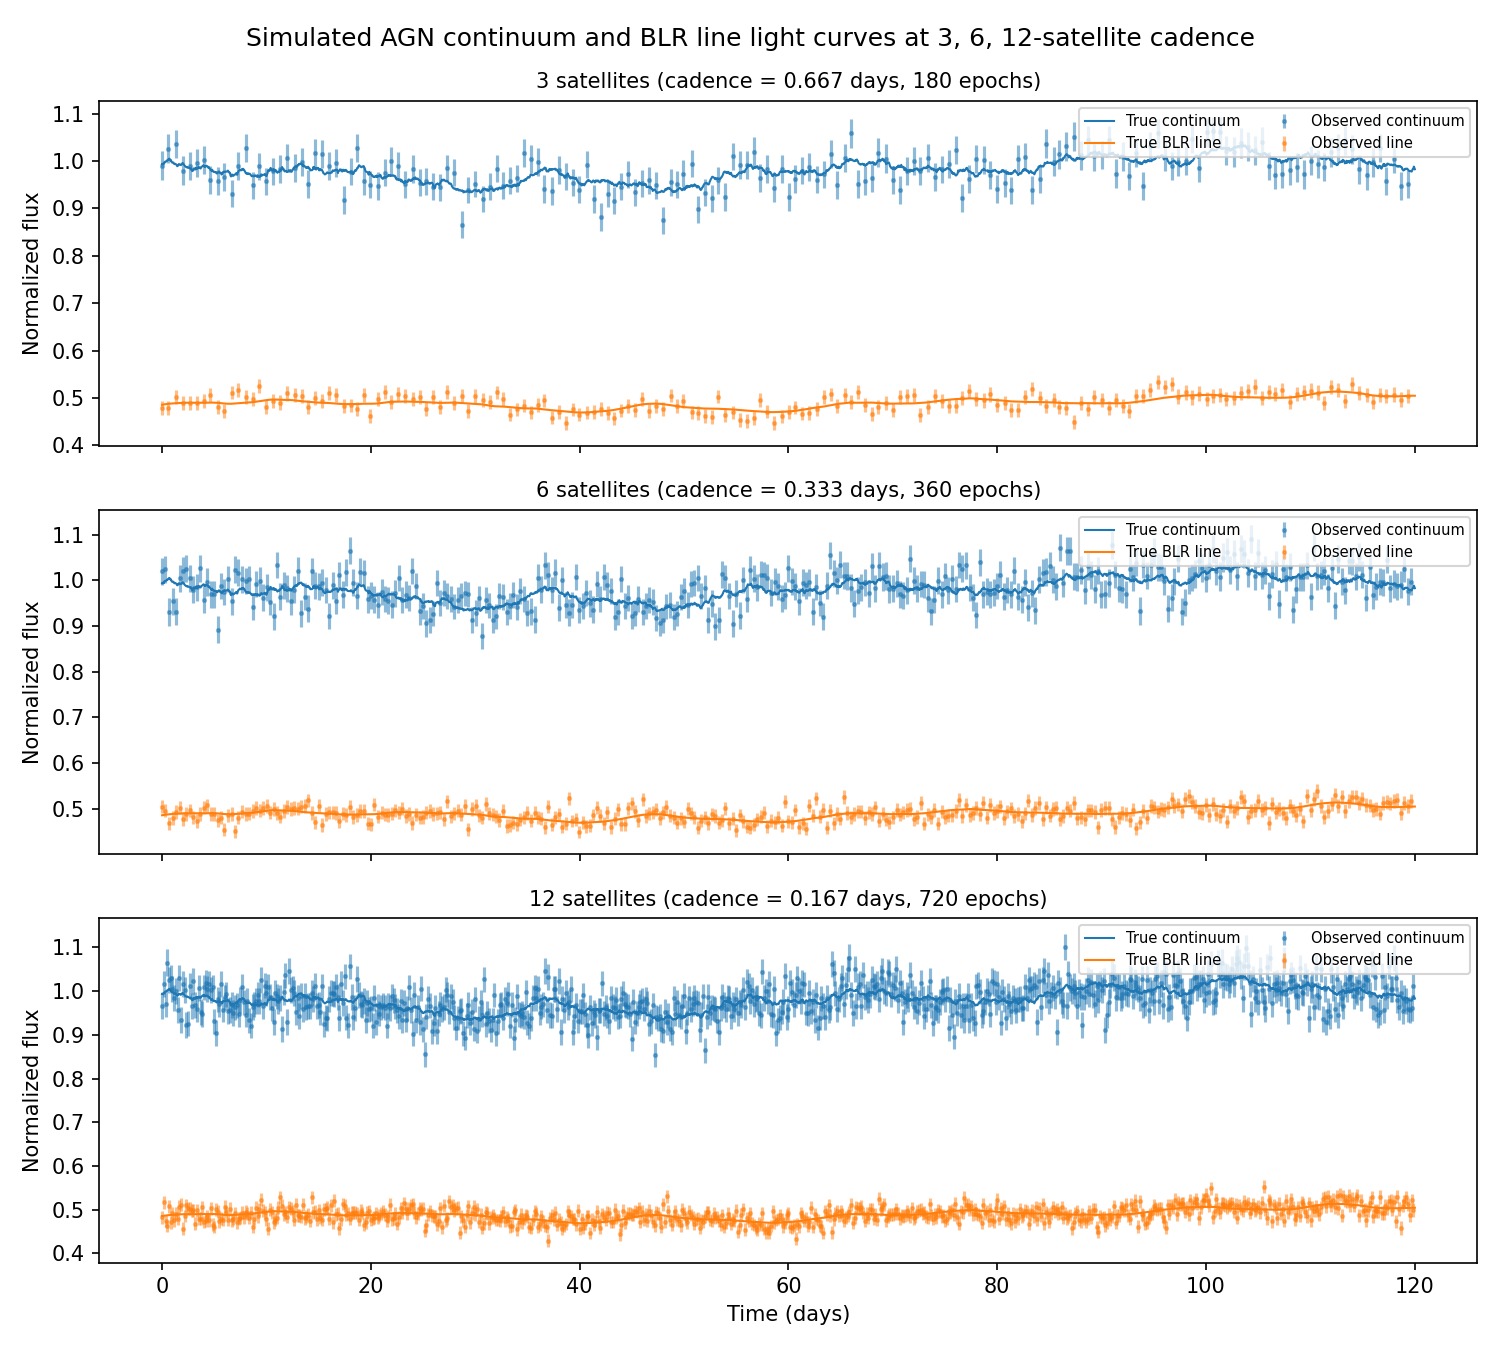
\includegraphics[width=0.85\textwidth]{fig1_example_light_curves.png}
\caption{Simulated AGN continuum (blue) and BLR line (orange) light curves for the same underlying realization, sampled at the 3-, 6-, and 12-satellite cadence. Solid lines show the true underlying light curve; markers with error bars show the noisy observed samples.}
\label{fig:lightcurves}
\end{figure}

\begin{figure}[htbp]
\centering
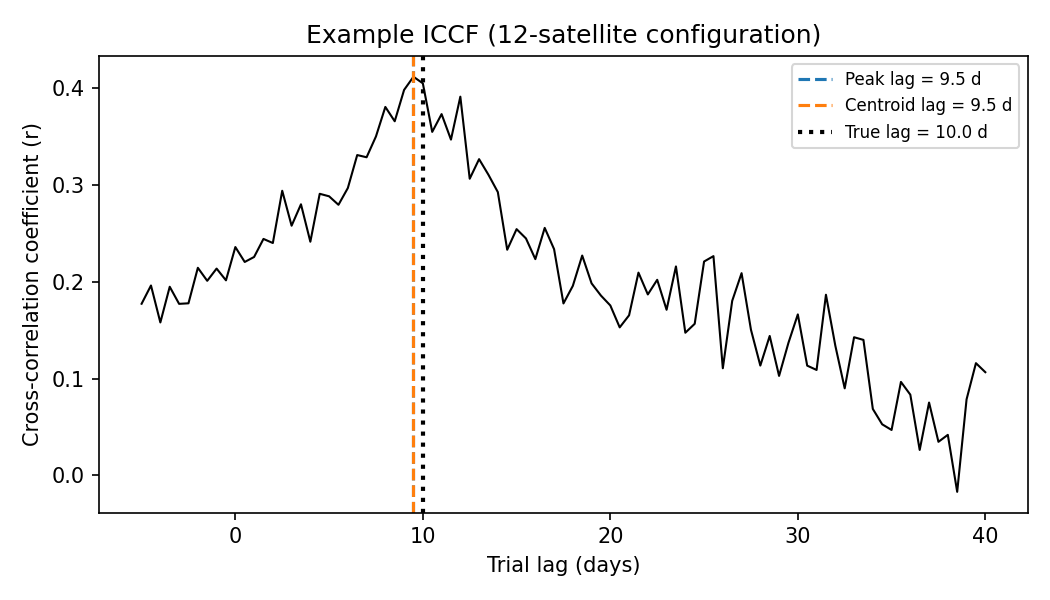
\includegraphics[width=0.7\textwidth]{fig2_example_ccf.png}
\caption{Example ICCF for the 12-satellite configuration, with peak lag, centroid lag, and true lag marked.}
\label{fig:ccf}
\end{figure}

\begin{figure}[htbp]
\centering
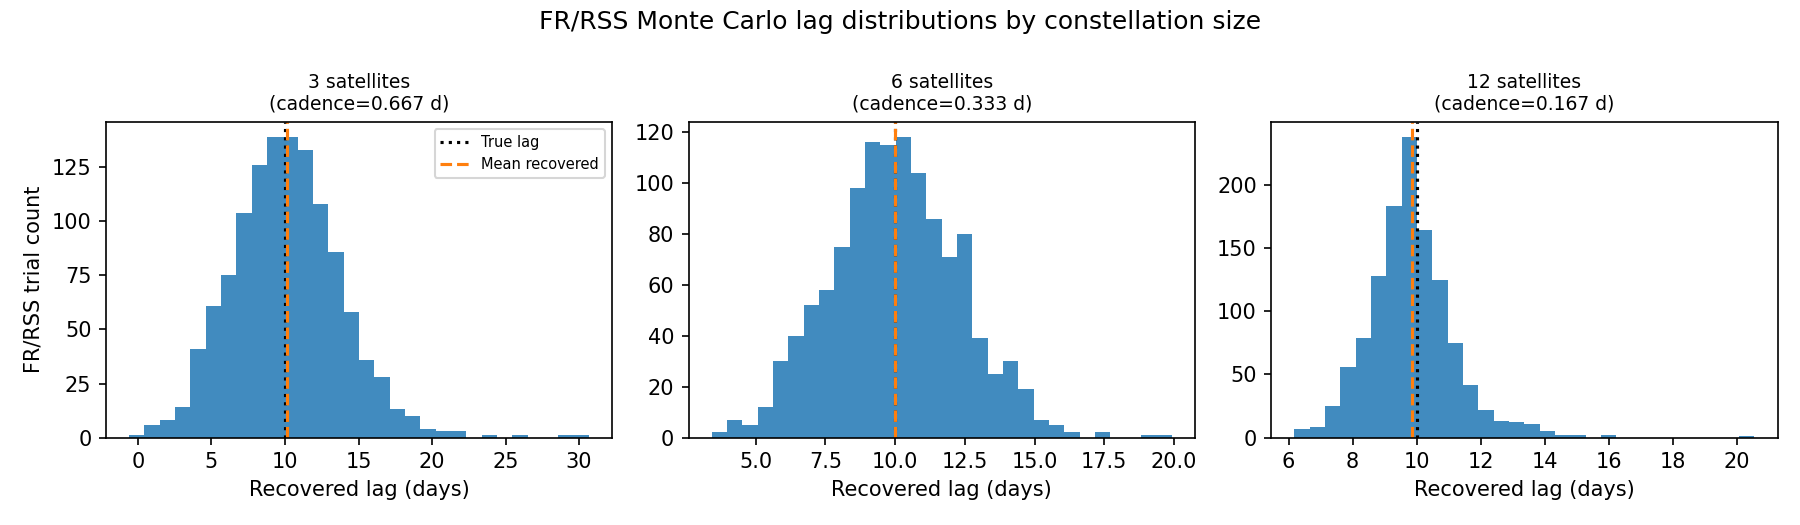
\includegraphics[width=0.95\textwidth]{fig3_frrss_distributions.png}
\caption{FR/RSS Monte Carlo lag distributions for a median-like realization at each constellation size, with the true lag and mean recovered lag marked.}
\label{fig:frrss}
\end{figure}

\subsection{Sensitivity to True Lag and Noise Level}

Figure~\ref{fig:combineduncertainty} and Tables~\ref{tab:lagsensitivity} and~\ref{tab:noisesensitivity} show that fractional lag uncertainty decreases monotonically with satellite count for all three true lags and is larger for shorter lags. For the 5-day lag the mean recovered lags (7.4 days at 3 satellites, 5.7 days at 12) exceed the true lag, so the fractional errors there are normalized by a biased lag. At every noise level 12 satellites give a lower uncertainty than 3, but the benefit shrinks as noise grows: at 6\% noise the step from 6 to 12 satellites is small (46.6\% to 42.5\%), and at 10\% noise it vanishes (48.2\% and 48.2\%). The dependence on noise is not strictly monotonic for 3 satellites (38.7\%, 54.2\%, 52.5\% at 3\%, 6\% and 10\%) because, at high noise, the correlation is weak and the centroid is biased toward long lags (mean recovered lags of 15.1 and 18.2 days at 6\% and 10\%), which deflates a fractional error normalized by the recovered lag.

\begin{figure}[htbp]
\centering
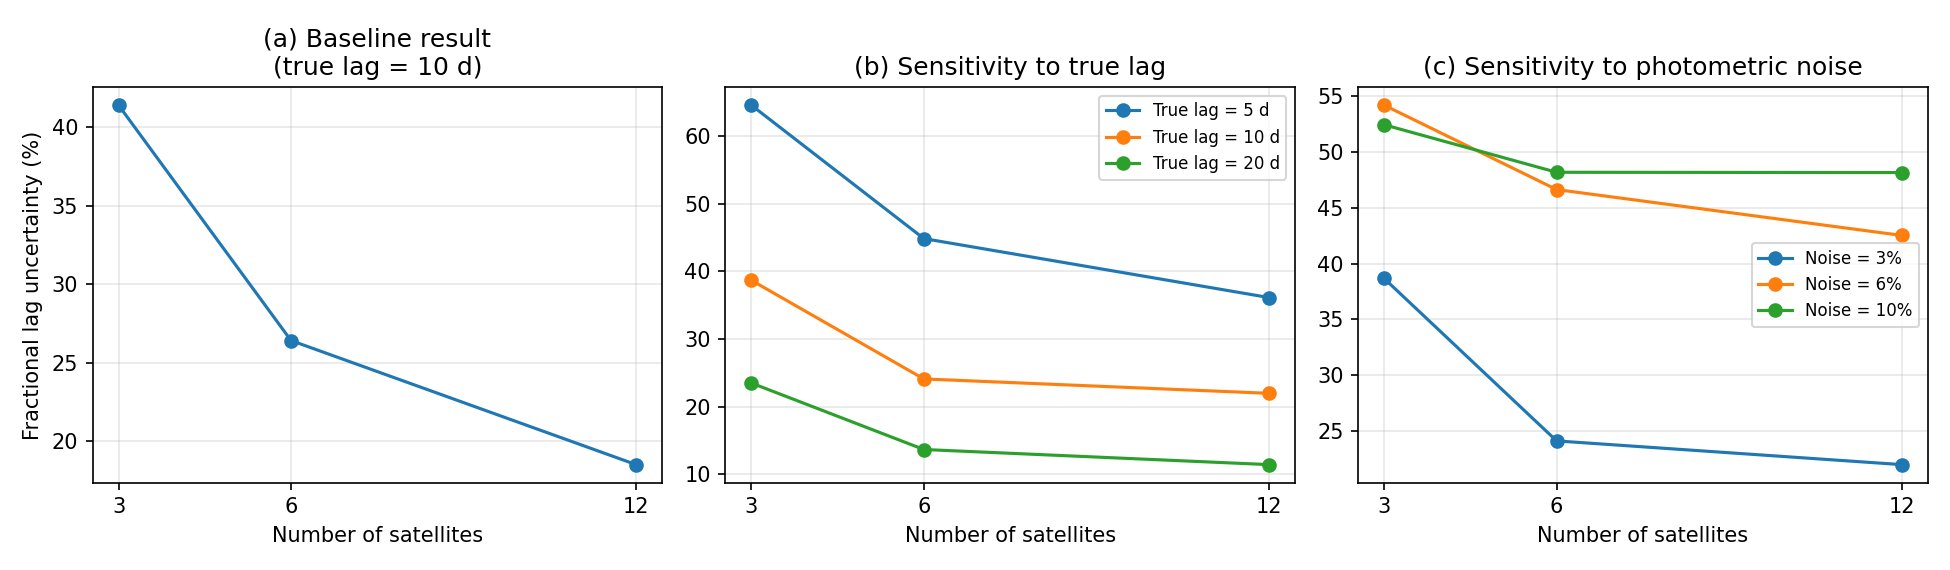
\includegraphics[width=\textwidth]{fig4_combined_uncertainty.png}
\caption{Fractional lag uncertainty versus constellation size. (a) Baseline (true lag 10 days, 100 realizations). (b) True lag of 5, 10 and 20 days (30 realizations). (c) Photometric noise of 3\%, 6\% and 10\% (30 realizations).}
\label{fig:combineduncertainty}
\end{figure}

\begin{table}[htbp]
\centering
\caption{Fractional lag uncertainty (mean recovered lag in parentheses) by true lag and constellation size (30 realizations per configuration).}
\label{tab:lagsensitivity}
\begin{tabular}{@{}cccc@{}}
\toprule
True lag & 3 satellites & 6 satellites & 12 satellites \\
\midrule
5 days & 64.5\% (7.4\,d) & 44.8\% (5.8\,d) & 36.1\% (5.7\,d) \\
10 days & 38.7\% (10.9\,d) & 24.1\% (10.4\,d) & 22.0\% (10.2\,d) \\
20 days & 23.5\% (19.1\,d) & 13.7\% (19.3\,d) & 11.5\% (18.7\,d) \\
\bottomrule
\end{tabular}
\end{table}

\begin{table}[htbp]
\centering
\caption{Fractional lag uncertainty (mean recovered lag in parentheses) by noise level and constellation size (30 realizations per configuration).}
\label{tab:noisesensitivity}
\begin{tabular}{@{}cccc@{}}
\toprule
Noise level & 3 satellites & 6 satellites & 12 satellites \\
\midrule
3\% & 38.7\% (10.9\,d) & 24.1\% (10.4\,d) & 22.0\% (10.2\,d) \\
6\% & 54.2\% (15.1\,d) & 46.6\% (13.7\,d) & 42.5\% (12.8\,d) \\
10\% & 52.5\% (18.2\,d) & 48.2\% (17.4\,d) & 48.2\% (16.1\,d) \\
\bottomrule
\end{tabular}
\end{table}

\subsection{Estimator Diagnostics}
\label{sec:diag}

Table~\ref{tab:diagnostics} reports the accuracy of the lag estimator against the known true lag. The FR/RSS uncertainty covers the true lag within $1\sigma$ in 81--92\% of realizations, higher than the 68\% expected for a Gaussian error, so it is somewhat conservative. The mean bias is small, with a 95\% interval that includes zero for 3 and 6 satellites and excludes it for 12 satellites, and gross failures are rare. Restricting the centroid to the contiguous region around the peak gives much larger fractional uncertainties (last column), so the absolute values depend on the centroid definition even though the ordering of the configurations does not.

\begin{table}[htbp]
\centering
\small
\caption{Accuracy of the ICCF centroid lag against the true lag (10 days), from the unperturbed light curves of 100 realizations per configuration (600 Monte Carlo trials). Bias is shown with its 95\% bootstrap interval; coverage is the fraction of realizations whose $1\sigma$ FR/RSS interval contains the true lag; failures are recovered lags more than 5 days from the truth. The last column is the fractional uncertainty with the centroid restricted to the contiguous region around the peak.}
\label{tab:diagnostics}
\begin{tabular}{@{}cccccc@{}}
\toprule
Satellites & Bias (days) & RMSE (days) & $1\sigma$ coverage & Gross failures & Frac. error, contiguous centroid \\
\midrule
3 & $-0.40$ ($-0.86$, $+0.05$) & 2.32 & 92\% & 5\% & 59.1\% \\
6 & $+0.17$ ($-0.21$, $+0.57$) & 1.98 & 88\% & 3\% & 41.2\% \\
12 & $-0.56$ ($-0.80$, $-0.33$) & 1.34 & 81\% & 0\% & 29.0\% \\
\bottomrule
\end{tabular}
\end{table}

The binning test (Table~\ref{tab:binning}) separates cadence from noise averaging. Averaging the 12-satellite data in groups of four gives 180 epochs, as for 3 satellites, with half the noise per point. The resulting lag uncertainty (1.58 days) is as small as that of the unbinned 12-satellite data (1.85 days) and far below that of the 3-satellite data (4.50 days). In the controlled experiment, therefore, the improvement from 3 to 12 satellites is explained by reduced photometric noise and not by the finer sampling interval, as expected for a smooth DRW signal, a 4-day transfer function and 3\% noise.

\begin{table}[htbp]
\centering
\small
\caption{Binning test: mean lag uncertainty ($\pm$ standard error) over 100 realizations.}
\label{tab:binning}
\begin{tabular}{@{}lc@{}}
\toprule
Configuration & Lag $\sigma$ (days) \\
\midrule
3 satellites (180 epochs, 3\% noise) & 4.50 $\pm$ 0.20 \\
12 satellites binned 4:1 to the 3-satellite cadence (180 epochs, 1.5\% noise) & 1.58 $\pm$ 0.08 \\
12 satellites (720 epochs, 3\% noise) & 1.85 $\pm$ 0.11 \\
\bottomrule
\end{tabular}
\end{table}

\subsection{Astrophysical Parameter Sweeps}
\label{sec:sweeps}

Table~\ref{tab:sweeps} and Figure~\ref{fig:sweeps} vary the DRW damping timescale, the variability amplitude and the transfer function in the controlled experiment, with and without a 36-day seasonal gap. Four results stand out. First, uncertainties grow with $\tau_d$: for 3 satellites with uniform sampling the fractional error rises from 23.7\% at 20 days to 38.3\% at 50 days and 53.2\% at 200 days, because slowly varying light curves contain less information on the lag timescale. Second, low-amplitude AGN are the hardest: at 1\% amplitude the uncertainty stays near 47.6\% even with 12 satellites and the recovered lag (17.3 days) is far from the true 10 days, i.e.\ lag recovery fails, whereas at 10\% and 15\% amplitude it falls to 5.2\% and 3.7\%. Third, skewed transfer functions raise the uncertainty and shift the recovered lag away from the true mean lag (for the log-normal with $\sigma = 4$~days the uncertainties are 43.5\%, 27.0\% and 20.4\%, with mean recovered lags of 11.8, 9.4 and 9.3 days for 3, 6 and 12 satellites, against a true mean lag of 10 days). Fourth, the seasonal gap raises the uncertainty everywhere and removes most of the benefit of additional satellites: in the fiducial case the 12-satellite uncertainty rises from 21.7\% to 42.6\%, and the gain from 3 to 12 satellites falls from 38.3\%--21.7\% to 50.3\%--42.6\%, with recovered lags of 12.3, 11.1 and 12.3 days. In relative terms the gap is most damaging for short damping timescales ($\tau_d = 20$~days: 10.8\% with uniform sampling versus 31.1\% with a gap, for 12 satellites), consistent with aliasing of faster variability across the gap.

\begin{table}[htbp]
\centering
\small
\caption{Fractional lag uncertainty (\%) for 3 / 6 / 12 satellites when one astrophysical parameter is varied (30 realizations, 400 Monte Carlo trials, 3\% noise). ``Gap'' removes epochs between days 41 and 77.}
\label{tab:sweeps}
\begin{tabular}{@{}lcc@{}}
\toprule
Setting & Uniform sampling & With seasonal gap \\
\midrule
DRW damping timescale $\tau_d$ = 20 d & 23.7 / 13.6 / 10.8 & 43.7 / 34.0 / 31.1 \\
$\tau_d$ = 50 d (fiducial) & 38.3 / 23.9 / 21.7 & 50.3 / 44.7 / 42.6 \\
$\tau_d$ = 100 d & 48.2 / 35.5 / 32.5 & 56.1 / 54.6 / 50.9 \\
$\tau_d$ = 200 d & 53.2 / 45.9 / 41.6 & 59.8 / 60.7 / 54.4 \\
Amplitude 1\% & 51.3 / 47.5 / 47.6 & 58.3 / 58.4 / 54.8 \\
Amplitude 4\% (fiducial) & 38.3 / 23.9 / 21.7 & 50.3 / 44.7 / 42.6 \\
Amplitude 10\% & 11.4 / 7.6 / 5.2 & 22.5 / 18.3 / 12.4 \\
Amplitude 15\% & 7.2 / 5.5 / 3.7 & 14.9 / 13.8 / 7.0 \\
Top-hat, width 4 d (fiducial) & 38.3 / 23.9 / 21.7 & 50.3 / 44.7 / 42.6 \\
Log-normal, $\sigma$ = 4 d & 43.5 / 27.0 / 20.4 & 54.5 / 47.0 / 44.7 \\
Log-normal, $\sigma$ = 8 d & 48.8 / 34.7 / 29.8 & 56.3 / 53.2 / 50.9 \\
\bottomrule
\end{tabular}
\end{table}

\begin{figure}[htbp]
\centering
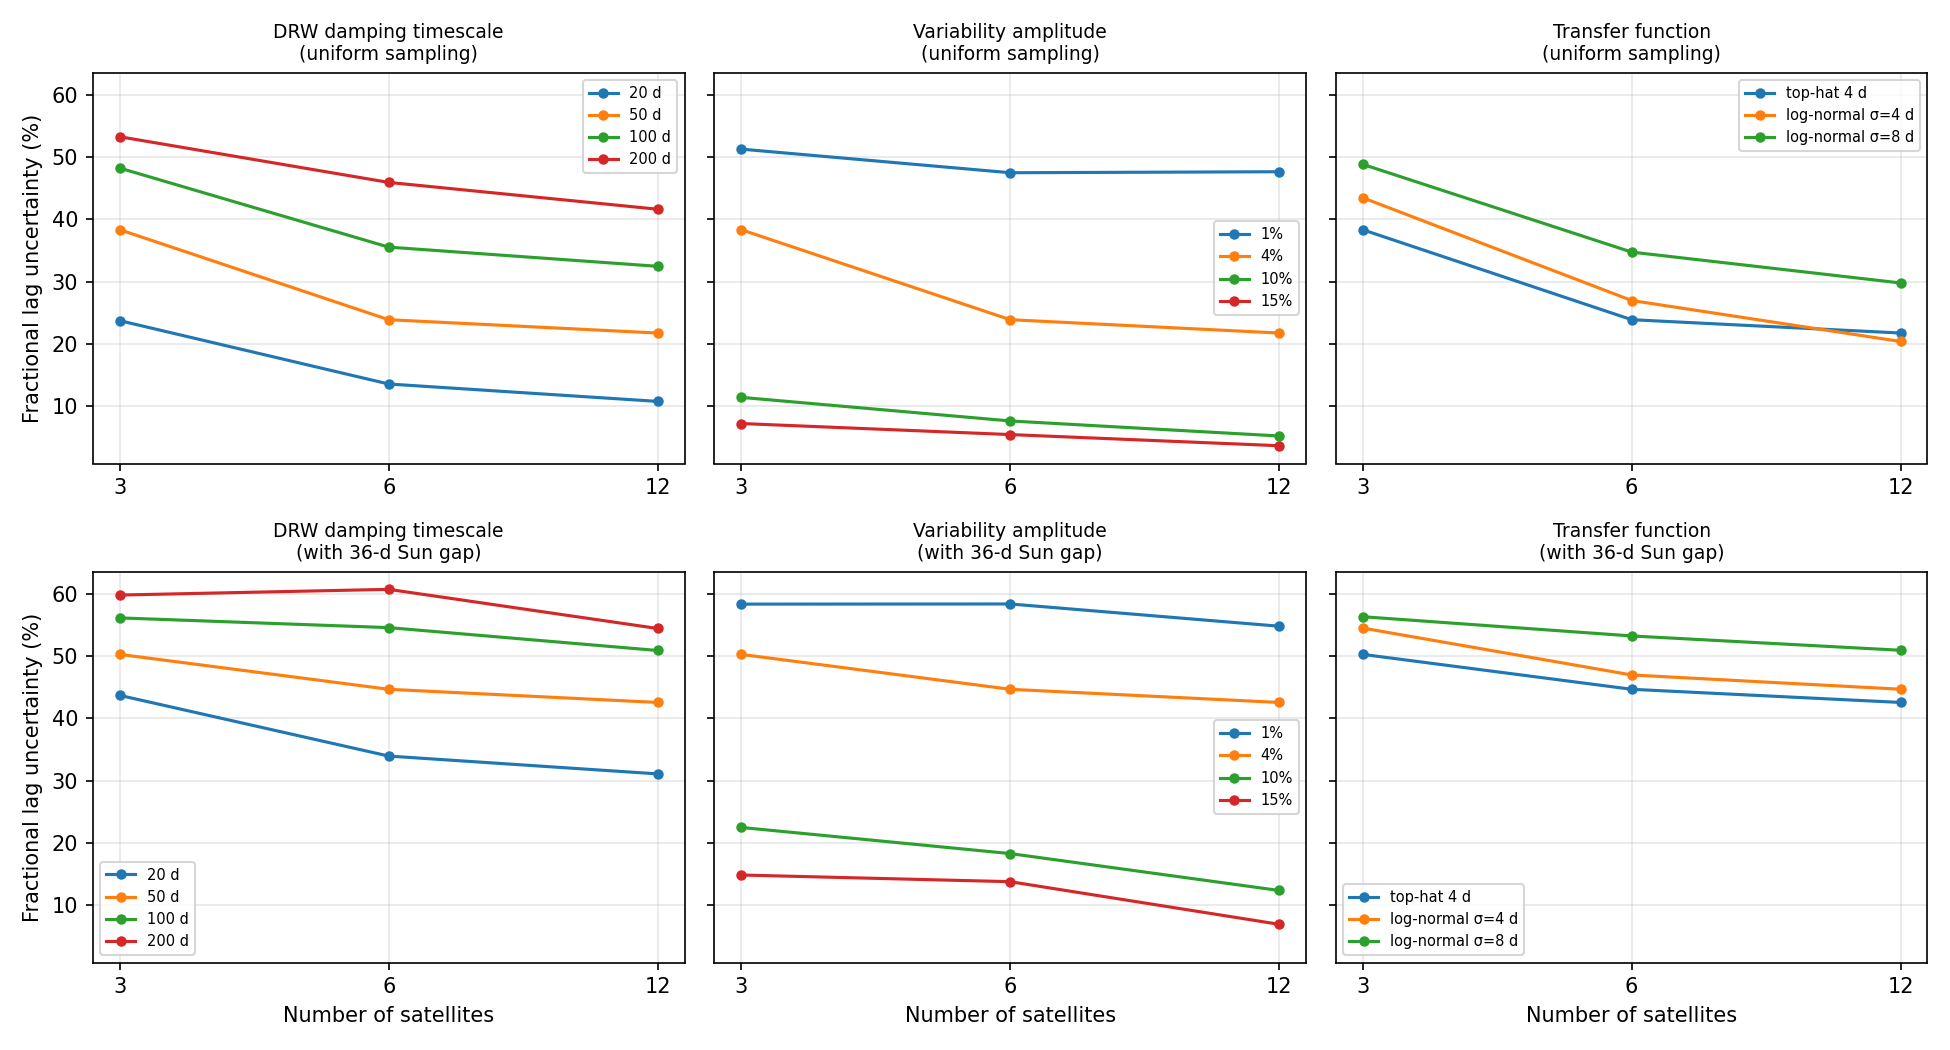
\includegraphics[width=\textwidth]{fig9_parameter_sweeps.png}
\caption{Fractional lag uncertainty versus constellation size when the DRW damping timescale, the variability amplitude or the transfer function is varied, for uniform sampling (top row) and with a 36-day seasonal gap (bottom row).}
\label{fig:sweeps}
\end{figure}

\subsection{Photon Budget and Achievable Cadence}
\label{sec:budget}

Table~\ref{tab:budget} gives the per-exposure noise of the representative photometer (120~s exposures). For a 10-cm aperture the continuum channel reaches 1.1\%, 1.9\%, 3.6\% and 7.6\% at $V = 14$, 15, 16 and 17, while the 150~\AA\ line channel reaches only 3.2\% to 28.8\%. Reaching 1\% in the continuum takes 147, 434, 1503 and 6397 seconds. A 15-cm aperture lowers the noise by a factor of about 1.5 (4.8\% at $V=17$).

\begin{table}[htbp]
\centering
\small
\caption{Per-exposure fractional photometric noise for 120~s exposures and exposure time needed to reach 1\% in the continuum channel (representative photometer; see Section~\ref{sec:instrument}).}
\label{tab:budget}
\begin{tabular}{@{}cccccc@{}}
\toprule
Aperture (cm) & $V$ & Continuum noise & Line-channel noise & Time for 1\% (s) \\
\midrule
10 & 14 & 1.1\% & 3.2\% & 147 \\
10 & 15 & 1.9\% & 6.0\% & 434 \\
10 & 16 & 3.6\% & 12.6\% & 1503 \\
10 & 17 & 7.6\% & 28.8\% & 6397 \\
15 & 14 & 0.7\% & 2.0\% & 64 \\
15 & 15 & 1.3\% & 3.6\% & 188 \\
15 & 16 & 2.3\% & 7.1\% & 637 \\
15 & 17 & 4.8\% & 15.5\% & 2646 \\
\bottomrule
\end{tabular}
\end{table}

With a cycle time of 180~s, a satellite could make 480 exposures per day if it could observe continuously, but Earth occultation, eclipses and (for some targets) the Sun limit the usable time, and the single station is in view for only about 39 minutes per day. For NGC~5548 a single satellite is limited by observing time to about 145 exposures per day, and downlink is not binding for photometric windows: 64~kB per exposure allows 127 exposures per day for one satellite and 1515 for twelve (Table~\ref{tab:downlink}). Downlinking full frames, however, limits a single satellite to 35 exposures per day and twelve satellites to 407, so the readout strategy can matter as much as the number of satellites. In all cases the achievable per-satellite cadence is much finer than the 2-day placeholder of the controlled experiment, which therefore understates what a single satellite can do.

\begin{table}[htbp]
\centering
\small
\caption{Exposures per day for NGC~5548 (V = 15) under the cycle-time (time-limited) and 2~Mbps downlink (bandwidth-limited) constraints for three data-volume strategies; the realised value is the smaller of the two.}
\label{tab:downlink}
\begin{tabular}{@{}cllcc@{}}
\toprule
Satellites & Data per exposure & Exposures per day & Time-limited & Bandwidth-limited \\
\midrule
1 & 64 kB cutouts & 127 & 145 & 9032 \\
1 & 1 MB windows & 124 & 145 & 578 \\
1 & 16 MB full frames & 35 & 145 & 35 \\
12 & 64 kB cutouts & 1515 & 1743 & 104503 \\
12 & 1 MB windows & 1477 & 1743 & 6689 \\
12 & 16 MB full frames & 407 & 1743 & 408 \\
\bottomrule
\end{tabular}
\end{table}

\subsection{Dynamic Orbits and Catalogued Targets}
\label{sec:targets}

\textbf{Solar exclusion.} Table~\ref{tab:targets} and Figure~\ref{fig:targets}a show how many of 120 days fall inside the $45^{\circ}$ Sun cone. Fairall~9 (ecliptic latitude $-59^{\circ}$) is never excluded, the mid-latitude targets NGC~5548, NGC~4151 and NGC~3783 lose up to 58 days, and the low-latitude targets NGC~7469 and Mrk~509 lose up to 87 and 88 days, with a longest single gap of 88 days. The excluded time depends strongly on when the campaign starts, from zero for a well-placed start to these maxima, so for low-latitude targets the campaign must be timed or extended over more than one season.

\textbf{Occultation and coverage.} With the precessing orbit, at least one satellite always has an unobstructed view of the target (Earth occultation alone leaves 100.0\% of the grid observable for every target and every constellation of 3 or more satellites), because the occulted fraction of an orbit is under half. For a campaign starting on 1 January 2026, the fraction of 0.5-day bins containing data is 85\% for NGC~5548 with one satellite and 91\% with twelve, but only 26\% for NGC~7469 and 35\% for Mrk~509 because their Sun gaps cover most of the campaign.

\textbf{Lag uncertainty.} At $V = 15$ and 4\% variability, a single satellite already reaches 6.2\% for NGC~5548, 6.8\% for NGC~3783 and 4.6\% for Fairall~9, and twelve satellites reach 2.8\%, 3.2\% and 3.0\%. The difference between constellation sizes is therefore modest, a few percentage points that are partly within the statistical noise of 30 realizations. For the low-latitude targets the uncertainty is far larger (31.8\% and 25.6\% with one satellite, 20.4\% and 17.8\% with twelve), and the recovered lag for Mrk~509 is biased high (14.7 days with one satellite and 13.1 days with twelve). Adding satellites reduces these uncertainties, but they remain large, whereas changing the campaign start date removes the gap altogether.

\begin{table}[htbp]
\centering
\small
\caption{Catalogued targets, campaign starting 1 January 2026 (V = 15, 4\% variability, 30 realizations, 600 trials). Excluded days are the minimum / mean / maximum over 12 campaign start dates; the longest single gap is the maximum over those starts; coverage is the fraction of 0.5-day bins with data for 12 satellites; the last four columns are the fractional lag uncertainty for 1, 3, 6 and 12 satellites.}
\label{tab:targets}
\resizebox{\textwidth}{!}{%
\begin{tabular}{@{}lccccccccc@{}}
\toprule
Target & Ecl.\ lat. & Excluded days & Longest gap (d) & Coverage & 1 sat & 3 sats & 6 sats & 12 sats \\
\midrule
NGC 4151 & $+37^{\circ}$ & 0 / 19 / 58 & 58 & 91\% & 6.1\% & 4.1\% & 3.3\% & 4.1\% \\
NGC 5548 & $+36^{\circ}$ & 0 / 19 / 58 & 58 & 91\% & 6.2\% & 4.4\% & 3.7\% & 2.8\% \\
NGC 7469 & $+14^{\circ}$ & 0 / 28 / 87 & 87 & 26\% & 31.8\% & 30.0\% & 22.9\% & 20.4\% \\
Mrk 509 & $+7^{\circ}$ & 0 / 28 / 88 & 88 & 35\% & 25.6\% & 21.3\% & 16.7\% & 17.8\% \\
NGC 3783 & $-36^{\circ}$ & 0 / 20 / 58 & 58 & 91\% & 6.8\% & 5.0\% & 3.1\% & 3.2\% \\
Fairall 9 & $-59^{\circ}$ & 0 / 0 / 0 & 0 & 91\% & 4.6\% & 3.3\% & 3.7\% & 3.0\% \\
\bottomrule
\end{tabular}}
\end{table}

\begin{figure}[htbp]
\centering
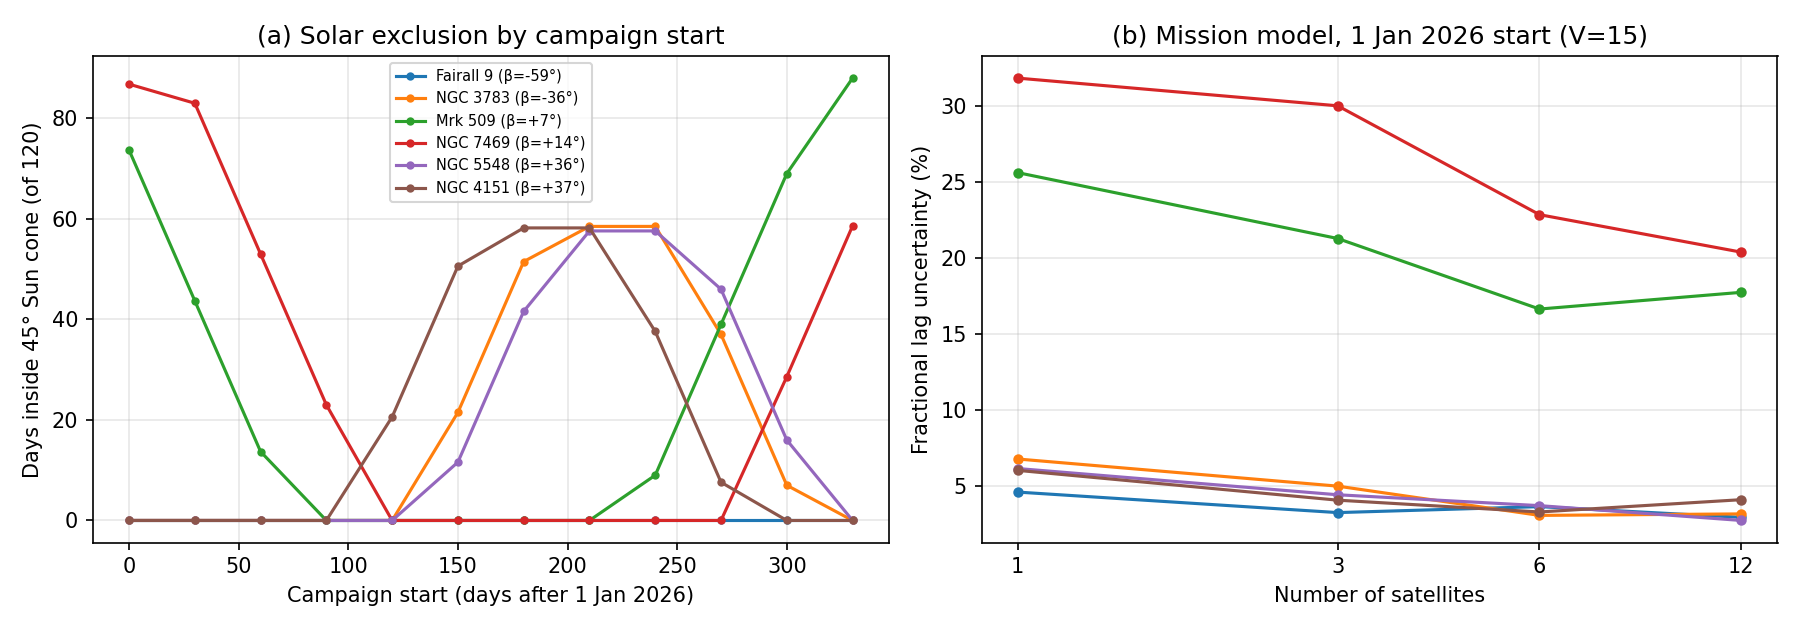
\includegraphics[width=\textwidth]{fig7_catalogue_targets.png}
\caption{(a) Days inside the 45$^{\circ}$ Sun cone for 120-day campaigns beginning on different dates, for six catalogued AGN (ecliptic latitude in the legend). (b) Fractional lag uncertainty versus constellation size for a campaign starting on 1 January 2026 (V = 15, 4\% variability).}
\label{fig:targets}
\end{figure}

\textbf{Brightness and variability.} Table~\ref{tab:mission} and Figure~\ref{fig:mission} show when constellation size matters. When photons are scarce the benefit is large: at $V = 17$ and 4\% variability the fractional lag uncertainty falls from 37.7\% with one satellite to 19.6\%, 11.5\% and 8.0\% with 3, 6 and 12. The same holds for weakly variable AGN: at $V = 15$ and 1\% variability it falls from 26.9\% to 7.0\%. For a bright target with strong variability ($V = 15$, 10\%) the uncertainty is already 3.4\% with one satellite and does not improve with more (3.1\% with twelve). The constellation size therefore matters when the lag signal is limited by photon noise, and not when it is limited by the AGN's own variability and by the observing window.

\begin{table}[htbp]
\centering
\small
\caption{Fractional lag uncertainty for NGC~5548 in the mission model, for different target magnitudes and variability amplitudes (campaign starting 1 January 2026, 30 realizations, 600 trials). The noise column is the median continuum noise per 0.5-day bin for 1 / 12 satellites.}
\label{tab:mission}
\begin{tabular}{@{}cccccccc@{}}
\toprule
$V$ & Amplitude & Bin noise (1 / 12 sat) & 1 sat & 3 sats & 6 sats & 12 sats \\
\midrule
15 & 4\% & 0.26\% / 0.08\% & 6.2\% & 4.4\% & 3.7\% & 2.8\% \\
16 & 4\% & 0.50\% / 0.15\% & 12.3\% & 6.7\% & 5.3\% & 5.1\% \\
17 & 4\% & 1.04\% / 0.31\% & 37.7\% & 19.6\% & 11.5\% & 8.0\% \\
15 & 1\% & 0.26\% / 0.08\% & 26.9\% & 12.5\% & 9.6\% & 7.0\% \\
15 & 10\% & 0.26\% / 0.08\% & 3.4\% & 3.0\% & 2.9\% & 3.1\% \\
17 & 10\% & 1.04\% / 0.31\% & 10.9\% & 6.1\% & 4.8\% & 4.1\% \\
\bottomrule
\end{tabular}
\end{table}

\begin{figure}[htbp]
\centering
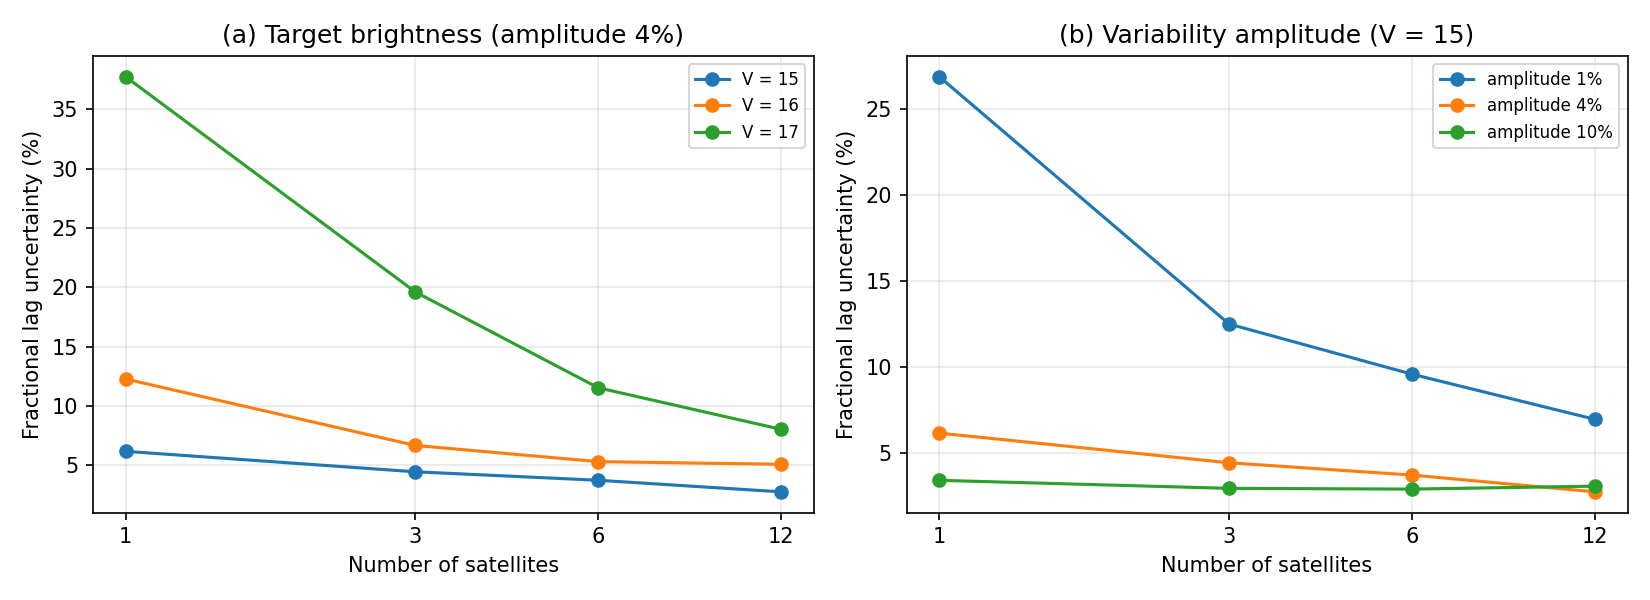
\includegraphics[width=0.95\textwidth]{fig8_mission_photon_budget.png}
\caption{Mission-model fractional lag uncertainty for NGC~5548 versus constellation size, for different target magnitudes (a) and variability amplitudes (b).}
\label{fig:mission}
\end{figure}

\section{Discussion}

In the controlled experiment, increasing the constellation from 3 to 12 satellites reduces the fractional lag uncertainty from 41.4\% to 18.5\%, consistent with the hypothesis, but the pattern is not the one the hypothesis expected. The absolute gain shrinks, yet the uncertainty falls roughly as $N^{-0.65}$ with no plateau, even though the 3-satellite cadence is already about 15 times finer than the 10-day lag, and the binning test shows that the improvement comes from averaging photometric noise over more epochs and not from a finer sampling interval. The field's rule of thumb that cadence finer than about five times the lag brings diminishing returns (Shablovinskaya et al., 2023) is therefore not what limits the precision here; what limits it is the number of photons collected.

This reading is reinforced by the mission model, in which noise and cadence are derived. A single 10-cm satellite already collects about 127 exposures per day for a mid-latitude target, far more than the 0.5 epochs per day implied by the 2-day placeholder, so the question changes from ``how fine can the cadence be?'' to ``how many photons does the lag measurement need?''. Constellation size helps when the photometry is the bottleneck (faint targets, low variability amplitude, or a narrow line channel) and does little when the intrinsic variability or the observing window is the bottleneck. In those cases a larger aperture, longer exposures or a different readout strategy may give the same improvement as additional satellites, and a constellation also adds redundancy, which is a separate benefit not quantified here.

The seasonal gap is the dominant limitation for low-ecliptic-latitude targets. It biases the recovered lag toward larger values, inflates the uncertainty, aliases fast variability, and removes most of the benefit of additional satellites, because the gap is the same for every satellite. High-ecliptic-latitude targets avoid it, and for targets within a few tens of degrees of the ecliptic the campaign start must be chosen, or the campaign extended over more than one season, to avoid it. This supports using target selection and campaign timing as design variables on a par with constellation size, and echoes the finding of Malik et al.\ (2022) and Malik (2023) that the observing window can matter more than cadence.

The sweeps show how far the results depend on the AGN: short damping timescales and large amplitudes are easier, low-amplitude AGN may not give a recoverable lag at all with 3\% noise and a 120-day baseline, and skewed transfer functions shift the centroid lag below the true mean lag. The reported percentages should therefore not be applied to a specific AGN without simulating its variability. The estimator diagnostics add that the all-lags centroid is conservative in its uncertainties but biased toward long lags when the correlation is weak, and that its uncertainties depend on the centroid definition.

Several limitations apply. The instrument parameters, ground station, downlink rate, data volume per exposure, thermal recovery time and Sun-avoidance angle are representative assumptions and not a specific design; the orbit is a single circular, 51.6$^{\circ}$ inclination orbit with one initial node, and we do not model Earth-limb avoidance, slewing between targets, pointing stability, radiation-belt passages or the South Atlantic Anomaly. All targets share one magnitude, one damping timescale and one transfer-function family per run, the line channel is treated without continuum contamination, and the 20\% velocity floor and the fixed virial factor mean that the mass uncertainties are statistical only (the systematic uncertainty in $f$, typically a few tenths of a dex, would exceed the differences between configurations). Finally, only the ICCF estimator was used. Methods that model the continuum as a Gaussian process, such as JAVELIN (Zu et al., 2011) and PyROA (Donnan et al., 2021), are standard in the field and generally handle irregular sampling and gaps better than linear interpolation; running them on these simulated light curves (the code repository provides an export tool) is the most important extension, because the conclusions about gaps and about faint, low-variability AGN may change with a better estimator.

\section{Conclusion}

We tested how CubeSat constellation size affects the uncertainty of reverberation-mapped lags and black hole masses for bright AGN with BLR lags of days to weeks. In a controlled experiment, increasing the constellation from 3 to 12 satellites reduced fractional lag uncertainty from 41.4\% to 18.5\% and mass uncertainty from 46.0\% to 27.2\% ($p<0.001$ for all pairwise comparisons); the uncertainty fell roughly as $N^{-0.65}$ without a plateau, and a binning test showed that the gain comes from averaging photometric noise over more epochs and not from finer sampling. In a mission-level model with a photon budget, a precessing orbit, a real solar ephemeris and six catalogued AGN, a single satellite already collects many exposures per day, and constellation size matters mainly for faint or weakly variable targets (for $V = 17$ the uncertainty falls from 37.7\% with one satellite to 8.0\% with twelve), not for bright, strongly varying ones. Solar exclusion depends on ecliptic latitude, from no exclusion at high latitude to gaps of up to 88 days near the ecliptic, and a seasonal gap biases the lag and removes most of the benefit of additional satellites. A low-cost constellation could therefore expand the set of AGN accessible to reverberation mapping, but target selection, campaign timing, aperture and data strategy matter at least as much as the number of satellites. Future work should compare ICCF with Gaussian-process estimators such as JAVELIN and PyROA, vary the orbit orientation and campaign start in the mission model, treat the line channel with continuum contamination, use measured magnitudes and variability properties for each target, and evaluate masses with a luminosity-calibrated radius--luminosity relation.

\section*{Code availability}

The simulation code, the results of every run reported here, and the script that generates this manuscript's tables and figures are available in the accompanying GitHub repository.
% TODO(author): add the repository URL here.

\section*{Acknowledgements}

The author thanks Dr. Ryan Farber for his mentorship and feedback throughout this research, including his guidance on strengthening the statistical rigor of the results.

\begin{thebibliography}{99}

\bibitem{eht2019}
Event Horizon Telescope Collaboration, Akiyama, K., Alberdi, A., et al. (2019). First M87 Event Horizon Telescope results. I. The shadow of the supermassive black hole. \textit{The Astrophysical Journal Letters, 875}(1), L1.

\bibitem{eht2022}
Event Horizon Telescope Collaboration, Akiyama, K., Alberdi, A., et al. (2022). First Sagittarius A* Event Horizon Telescope results. I. The shadow of the supermassive black hole in the center of the Milky Way. \textit{The Astrophysical Journal Letters, 930}(2), L12.

\bibitem{gorjian2025}
Gorjian, V., Ardila, D., Barth, A., et al. (2025). UV/optical active galactic nuclei reverberation mapping: Using a SmallSat to trade time resolution for spatial resolution to study accretion disks around supermassive black holes at the centers of galaxies. \textit{Journal of Astronomical Telescopes, Instruments, and Systems, 11}(4), 042226.

\bibitem{kelly2009}
Kelly, B. C., Bechtold, J., \& Siemiginowska, A. (2009). Are the variations in quasar optical flux driven by thermal fluctuations? \textit{The Astrophysical Journal, 698}(1), 895--910.

\bibitem{knapp2018}
Knapp, M., Seager, S., et al. (2018). On the verge of an astronomy CubeSat revolution. \textit{Nature Astronomy, 2}, 358--367.

\bibitem{lewin2025}
Lewin, C. (2025). \textit{Reverberation mapping of supermassive black holes using machine learning} [Doctoral thesis, Massachusetts Institute of Technology]. MIT DSpace. \url{https://hdl.handle.net/1721.1/164512}

\bibitem{malik2023}
Malik, U. (2023). \textit{Supermassive black hole masses with multi-object reverberation mapping} [Doctoral dissertation, The Australian National University]. ProQuest Dissertations \& Theses. 31855562.

\bibitem{obswindow2022}
Malik, U., Sharp, R., Martini, P., Davis, T. M., Tucker, B. E., Yu, Z., Penton, A., Lewis, G. F., \& Calcino, J. (2022). Observational window effects on multi-object reverberation mapping. arXiv:2203.04518.

\bibitem{miller2026}
Miller, J. A., Cackett, E. M., Bentz, M. C., Goad, M. R., Korista, K. T., McHardy, I. M., \& Carroll, R. W. (2026). Continuum reverberation mapping of 18 active galactic nuclei over 4 yr. \textit{The Astrophysical Journal}.

\bibitem{onken2004}
Onken, C. A., Ferrarese, L., Merritt, D., Peterson, B. M., Pogge, R. W., Vestergaard, M., \& Wandel, A. (2004). Supermassive black holes in active galactic nuclei. II. Calibration of the black hole mass-velocity dispersion relationship for active galactic nuclei. \textit{The Astrophysical Journal, 615}(2), 645--651.

\bibitem{peterson1998}
Peterson, B. M., Wanders, I., Horne, K., Collier, S., Alexander, T., Kaspi, S., \& Maoz, D. (1998). On uncertainties in cross-correlation lags and the reality of wavelength-dependent continuum lags in active galactic nuclei. \textit{Publications of the Astronomical Society of the Pacific, 110}(750), 660--670.

\bibitem{peterson2004}
Peterson, B. M., Ferrarese, L., Gilbert, K. M., Kaspi, S., Malkan, M. A., Maoz, D., Merritt, D., Netzer, H., Onken, C. A., Pogge, R. W., Vestergaard, M., \& Wandel, A. (2004). Central masses and broad-line region sizes of active galactic nuclei. II. A homogeneous analysis of a large reverberation-mapping database. \textit{The Astrophysical Journal, 613}(2), 682--699.

\bibitem{shablovinskaya2023}
Shablovinskaya, E., Popovi\'{c}, L. \v{C}., Uklein, R., Malygin, E., Ili\'{c}, D., Ciroi, S., Oparin, D., Crepaldi, L., Slavcheva-Mihova, L., Mihov, B., \& Nikolov, Y. (2023). Polarimetric reverberation mapping in medium-band filters. \textit{Universe, 9}(1), 52.

\bibitem{vallado2013}
Vallado, D. A. (2013). \textit{Fundamentals of Astrodynamics and Applications} (4th ed.). Microcosm Press.

\bibitem{zu2011}
Zu, Y., Kochanek, C. S., \& Peterson, B. M. (2011). An alternative approach to measuring reverberation lags in active galactic nuclei. \textit{The Astrophysical Journal, 735}(2), 80.

\bibitem{donnan2021}
Donnan, F. R., Horne, K., \& Hern\'{a}ndez Santisteban, J. V. (2021). PyROA: a Python package for flexible modelling of AGN light curves. \textit{Monthly Notices of the Royal Astronomical Society, 508}(4), 5449--5461.

\bibitem{white1994}
White, R. J., \& Peterson, B. M. (1994). Comments on cross-correlation methodology in variability studies of active galactic nuclei. \textit{Publications of the Astronomical Society of the Pacific, 106}(701), 879--889.

\end{thebibliography}

\end{document}
